%%%%%%%%%%%%%%%%%%%%%%%%%%%%%%%%%%%%%%%%%
% Frequently Asked Questions
% LaTeX Template
% Version 1.0 (22/7/13)
%
% This template has been downloaded from:
% http://www.LaTeXTemplates.com
%
% Original author:
% Adam Glesser (adamglesser@gmail.com)
%
% License:
% CC BY-NC-SA 3.0 (http://creativecommons.org/licenses/by-nc-sa/3.0/)
%
%%%%%%%%%%%%%%%%%%%%%%%%%%%%%%%%%%%%%%%%%

\documentclass[11pt]{article}

\usepackage[margin=1in]{geometry} % Required to make the margins smaller to fit more content on each page
\usepackage[linkcolor=blue]{hyperref} % Required to create hyperlinks to questions from elsewhere in the document
\hypersetup{pdfborder={0 0 0}, colorlinks=true, urlcolor=blue} % Specify a color for hyperlinks
\usepackage{todonotes} % Required for the boxes that questions appear in
\usepackage{tocloft} % Required to give customize the table of contents to display questions
\usepackage{microtype} % Slightly tweak font spacing for aesthetics
\usepackage{palatino} % Use the Palatino font
\usepackage{cite}
\usepackage{float}

\setlength\parindent{0pt} % Removes all indentation from paragraphs

% Create and define the list of questions
\newlistof{questions}{faq}{\large List of Frequently Asked Questions} % This creates a new table of contents-like environment that will output a file with extension .faq
\setlength\cftbeforefaqtitleskip{4em} % Adjusts the vertical space between the title and subtitle
\setlength\cftafterfaqtitleskip{1em} % Adjusts the vertical space between the subtitle and the first question
\setlength\cftparskip{.3em} % Adjusts the vertical space between questions in the list of questions

% Create the command used for questions
\newcommand{\question}[1] % This is what you will use to create a new question
{
\refstepcounter{questions} % Increases the questions counter, this can be referenced anywhere with \thequestions
\par\noindent % Creates a new unindented paragraph
\phantomsection % Needed for hyperref compatibility with the \addcontensline command
\addcontentsline{faq}{questions}{#1} % Adds the question to the list of questions
\todo[inline, color=green!40]{\textbf{#1}} % Uses the todonotes package to create a fancy box to put the question
\vspace{1em} % White space after the question before the start of the answer
}

% Uncomment the line below to get rid of the trailing dots in the table of contents
%\renewcommand{\cftdot}{}

% Uncomment the two lines below to get rid of the numbers in the table of contents
%\let\Contentsline\contentsline
%\renewcommand\contentsline[3]{\Contentsline{#1}{#2}{}}

\begin{document}

%----------------------------------------------------------------------------------------
%	TITLE AND LIST OF QUESTIONS
%----------------------------------------------------------------------------------------

\begin{center}
\Huge{\bf \emph{Autonomous Driving Simulation Topics and Ideas}} % Main title
\end{center}

\listofquestions % This prints the subtitle and a list of all of your questions

\newpage % Comment this if you would like your questions and answers to start immediately after table of questions

\section{Introduction}

\section{Behavior Simulation}
\subsection{Crowd Simulation}
\subsection{Pedestrian Animation}
\question{What are some references around basic pedestrian simulation?}

\paragraph{Koopman et al. 1995 \cite{Koopman1995}}

Koopman et al. 1995 \cite{Koopman1995} have described an inverse dynamics model for animation reconstruction and prediction of bipedal motion.


\begin{figure}[H]
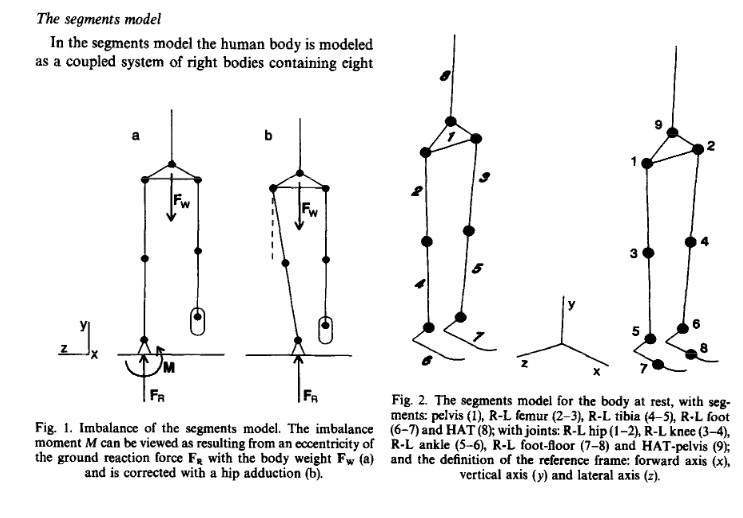
\includegraphics[width=0.9\textwidth]{images/koopman_segments.png}
\caption{Koopman et al. \cite{Koopman1995} bipedal model consisting of segmented rigid bodies}
\end{figure}

Overall ideas from \cite{Koopman1995}:
\begin{itemize}
\item rigid body segments with frames oriented across principal directions
\item 3DOF spherical joints / ball hinges
\item joint translations are possible, but are a function of the rotation parameters
\item the inverse dynamics problem is solved by assuming the rotation angle profiles to be approximated via
Fourier series; their coefficients are then treated as optimization variables
\item joint angle measurements are gathered from several subjects and the walk cycles are averaged!
\item kinematic constraints are solved for to yield additional joint angles
\end{itemize}

\begin{figure}[H]
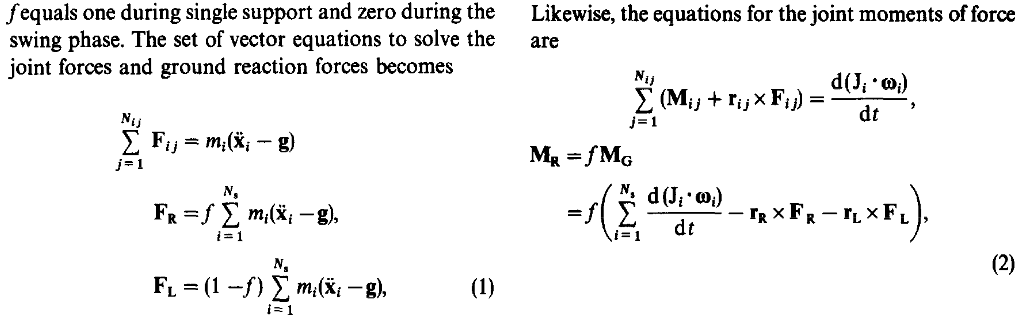
\includegraphics[scale=0.5]{images/koopman_equations.png}
\caption{Koopman et al. \cite{Koopman1995} left and right foot dynamics equations}
\end{figure}

\paragraph{Kuo 2007 \cite{Kuo2007}}

\begin{figure}[H]
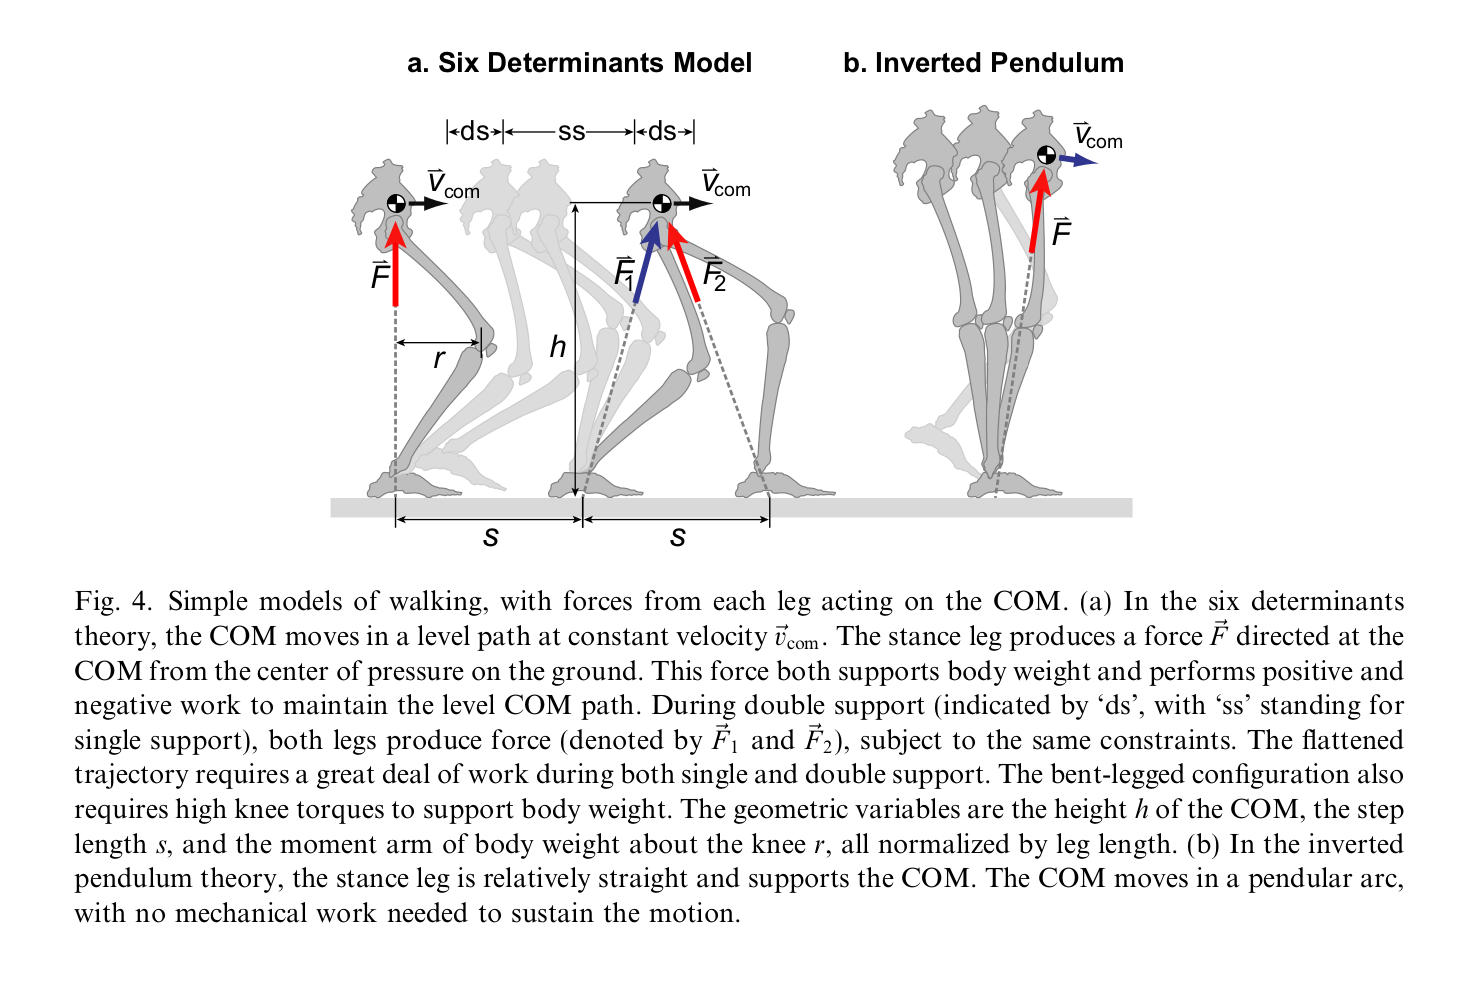
\includegraphics[width=0.9\textwidth]{images/kuo_inv_pendulum.png}
\caption{Kuo \cite{Kuo2007} compared the six determinants model to a more natural inverted pendulum model}
\end{figure}

\paragraph{Seitz et al 2014 \cite{Seitz2014}}

From Seitz et al 2014 \cite{Seitz2014}:
"For instance, pedestrians are simulated as an inverted pendulum Kuo 2007 \cite{Kuo2007}"
Seitz et al. \cite{Seitz2014} analyzed different walking modes (slow, medium, fast, with/out obstacles, with/out stop/resume) to understand how the pace and the step size differs and what trajectories the pedestrians usually prefer. 

\begin{figure}[H]
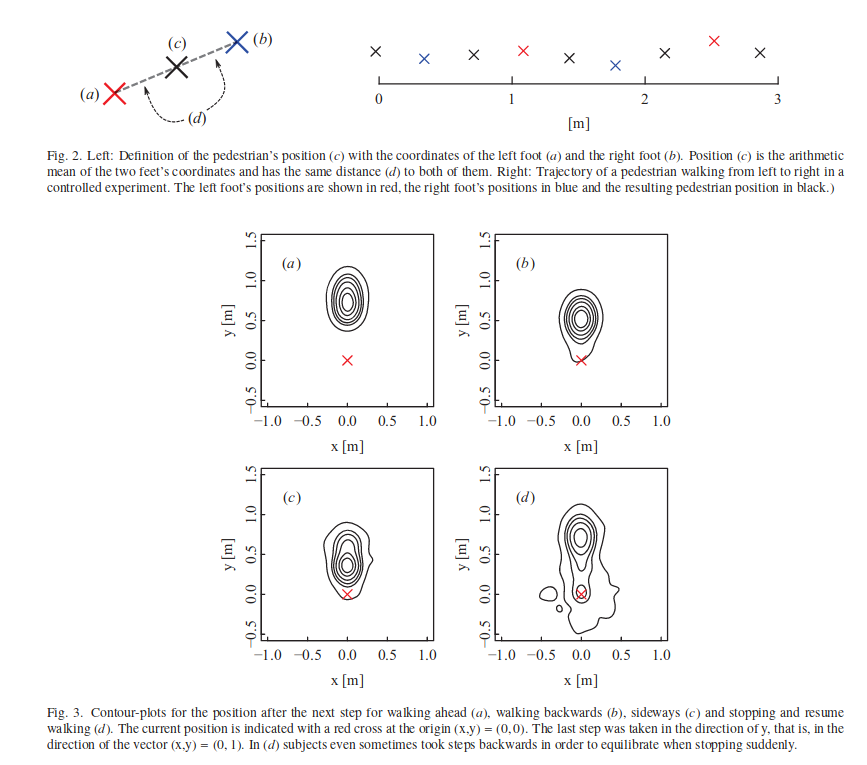
\includegraphics[width=0.9\textwidth]{images/steitz_steps_distribution.png}
\end{figure}

\begin{figure}[H]
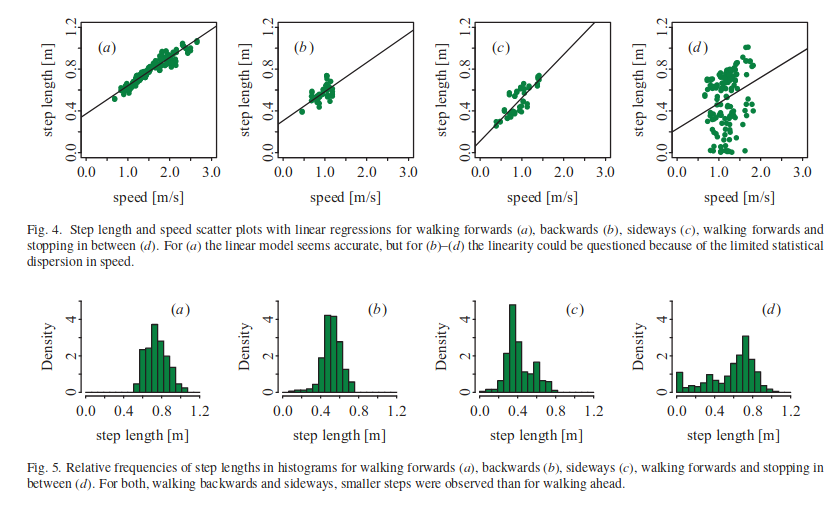
\includegraphics[width=0.9\textwidth]{images/steitz_speed_vs_step_size.png}
\end{figure}


\subsection{Vehicle Behavior Simulation}

\section{Sensors and Environment Simulation}
\subsection{LiDAR Simulation}
\subsection{Radar Simulation}



%----------------------------------------------------------------------------------------
%	QUESTIONS AND ANSWERS
%----------------------------------------------------------------------------------------

\question{How do I add a new question and answer?}\label{new-question}

In the code, type:

\begin{verbatim}
\question{A question that needs answering}\label{question-label}

The answer to this question.
\end{verbatim}

%------------------------------------------------

\question{Why is there a label in the code for \hyperref[new-question]{the previous question}?}\label{labels}

This is not necessary, but it does give you a way of linking to a different question. In order to link to another question you simply need to add the following:

\begin{verbatim}
\hyperref[question-label]{click here}
\end{verbatim}

The first part \texttt{[question-label]} is the label name and the second part \texttt{\{click here\}} is the text that is displayed as link.

%------------------------------------------------

\question{How do I change the title and subtitle?}\label{change-title}

To change the main title, simply find the "TITLE AND LIST OF QUESTIONS" block and replace "A Template for FAQ's" within it. To change the subtitle find the following command:

\begin{verbatim}
\newlistof{questions}{faq}{\large List of Frequently Asked Questions}
\end{verbatim}

and replace the subtitle with one of your choosing.

%------------------------------------------------

\question{Is it possible to change the spacing between the questions in the list of questions?}\label{change-spacing}

Yes, simply find the following line:

\begin{verbatim}
\setlength\cftparskip{.3em}
\end{verbatim}

and change the \texttt{.3em} to whatever suits your fancy.

%------------------------------------------------

\question{What if I want to hide the page numbers and/or trailing dots next to the question in the list of questions?}\label{page-numbering}

To remove the trailing dots to the page numbers, find the line:

\begin{verbatim}
%\renewcommand{\cftdot}{}
\end{verbatim}
and uncomment it. To remove the page numbers as well, find the following lines and uncomment them:
\begin{verbatim}
%\let\Contentsline\contentsline
%\renewcommand\contentsline[3]{\Contentsline{#1}{#2}{}}
\end{verbatim}

%------------------------------------------------

\question{Is it possible to number questions?}\label{number-questions}

Yes, you can refer to the number of the current question with:

\begin{verbatim}
\thequestions
\end{verbatim}
 
For example, this is question \thequestions. You can even incorporate question numbers into the questions and list of questions automatically by adding:

\begin{verbatim}
Question \thequestions:
\end{verbatim}

just before each \texttt{\#1} in the \texttt{\textbackslash questions} definition block in the preamble.

%------------------------------------------------

\question{Question \thequestions: Can I change the color of the question boxes?}\label{question-color}

Just find the following line and change the color specified there:

\begin{verbatim}
\todo[inline, color=green!40]{\textbf{#1}}
\end{verbatim}

%----------------------------------------------------------------------------------------



\medskip
\nocite{*}
\bibliographystyle{plain}
\bibliography{sim}



\end{document}
